%%% Preamble starts here.
\documentclass{amsart}
%for the heading
\usepackage{fancyhdr,gensymb, enumerate,multirow,float}
%for the picture. 
\usepackage{tikz, calc}
%adjust the page width
\usepackage[margin=1in]{geometry}

\usepackage{array}   % for \newcolumntype macro
\newcolumntype{L}{>{$}l<{$}} % math-mode version of "l" column type


%% The next line says how the "vertex" style of nodes should look: drawn as small circles.
\tikzstyle{vertex}=[circle, draw, inner sep=0pt, minimum size=6pt,fill=white]
%%
%% Next, we make a \vertex command as a shorthand in place of \node[vertex} to get that style.
\newcommand{\vertex}{\node[vertex]}

\linespread{1.1}


%special commands for number sets
\def\RR{{\mathbb R}}
\def\NN{{\mathbb N}}
\def\ZZ{{\mathbb Z}}
\def\QQ{{\mathbb Q}}
\def\CC{{\mathbb C}}

% header
\lhead{\sc  Senior Seminar: Homework 10}
\chead{\sc Stefano Fochesatto } 
\rhead{due: Friday 04/10/2020}
\cfoot{}
\pagestyle{fancy}

%%%% Main document starts here.

\begin{document}
\thispagestyle{fancy}
 
\begin{enumerate}
\item (Problem A:) For the graphs $G_1$ and $G_2$ below, describe the automorphisms of $G_1$ and $G_2$ in terms of permutation cycles. Explain why your answer is correct. (See Figure 2.3 on page 39 of the handout for an example of the automorphisms of $C_4$ described in terms of permutation cycles.) \\

\begin{center}
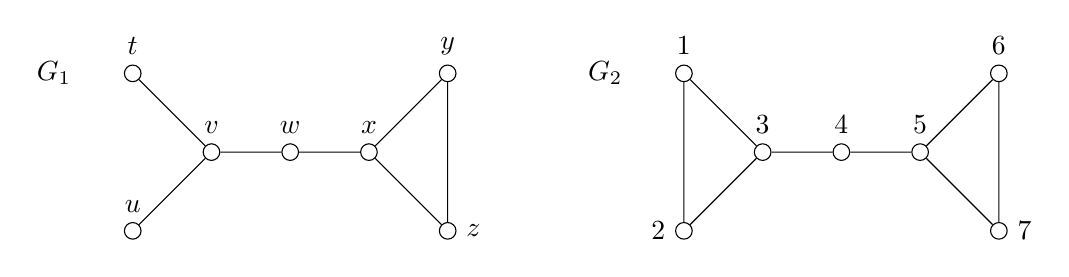
\begin{tikzpicture}
\node at (-1,1){$G_1$};
\vertex (t) at (0,1)[label=above:{$t$}]{};
\vertex (u) at (0,-1)[label=above:{$u$}]{};
\vertex (v) at (1,0)[label=above:{$v$}]{};
\vertex (w) at (2,0)[label=above:{$w$}]{};
\vertex (x) at (3,0)[label=above:{$x$}]{};
\vertex (y) at (4,1)[label=above:{$y$}]{};
\vertex (z) at (4,-1)[label=right:{$z$}]{};
\draw (t)--(v)--(u)(v)--(w)--(x)--(y)--(z)--(x);
\node at (6,1){$G_2$};
\vertex (1) at (7,1)[label=above:{$1$}]{};
\vertex (2) at (7,-1)[label=left:{$2$}]{};
\vertex (3) at (8,0)[label=above:{$3$}]{};
\vertex (4) at (9,0)[label=above:{$4$}]{};
\vertex (5) at (10,0)[label=above:{$5$}]{};
\vertex (6) at (11,1)[label=above:{$6$}]{};
\vertex (7) at (11,-1)[label=right:{$7$}]{};
\draw (3)--(2)--(1)--(3)--(4)--(5)--(6)--(7)--(5);
\end{tikzpicture}
\end{center}

\textbf{Answer:}\\
$Aut(G_1) = \{\epsilon, (ut),(yz),(ut)(yz)\}$ We can see that the function $(ut)$ preserves (non)-adjacency and similarly with $(yz)$. Since $Aut(G_1)$ is a group it must be closed under function composition $(ut)(yz)$ must also be included. \\\\
$Aut(G_2) = \{\epsilon, (12),(67),(12)(67), (16)(27)(35), (17)(62)(35), (1627)(35), (1726)(34)\}$ This whole group can be composed from a set of 3 base permutation $\{(12),(67),(16)(27)(35), \epsilon\}$, which correspond to the symmetries on the graph. I can't seem to find any more reflection symmetries and any rotational symmetry is a composition the reflection symmetries I listed before.   









\vspace{1.5in}

\item (Problem B) Prove that for $n\geq 3,$ $Aut(C_n) \cong D_n$ where $D_n$ is the dihedral group with $2n$ elements.  \\


\textbf{Answer:} The dihedral group is defined as the group of symmetries of a regular polygon. We know that $|D_n| = 2n$ we get $n$ from the rotational symmetries and $n$ from reflection symmetries. Reflection symmetries are different depending on the parity of $n$. When $n$ is odd the axis of reflection is always between a vertex and the midpoint of the opposite edge. When $n$ is even the axis of reflection is either between two opposite vertices or two opposite edges. From here it clear that for cases $n\leq 2$ the symmetries are trivial. The isomorphism comes from the idea that any $C_n$ can be redrawn as an $n$-vertex regular polygon and therefore contains the same symmetries. Since every permutation in $Aut(C_n)$ can be described with a symmetry or composition of symmetries we get that the groups are the same.\\\\




This is my attempt at an isomorphism proof.\\
\textbf{Proof:} Consider the isomorphism $f: Aut(C_n) \to D_n$, such that $f(i) = i$.\\

Injection: Suppose $a,b \in Aut(C_n)$ such that $f(a) = f(b)$. By the definition $D_n$ we know that $f(b)$ and $f(a)$ correspond to the same symmetry of an $n$-vertex regular polygon. Note that $Aut(C_n)$ contains (non)-adjacency preserving permutations of the set $V(C_n)$ and any $C_n$ can be redrawn as an $n$-vertex regular polygon. 
Since we know that there is an injective correspondence between symmetries and permutations it must be the case that $a = b$.\\

Surjection: Suppose $b \in D_n$. Let $a$ be the permutation in $Aut(C_n)$ which corresponds to the symmetry $b$. Thus $f(a) = b$.\\

Homomorphism: Suppose $f(ab)$ where $a,b \in Aut(C_n)$. By definition $f(ab) = ab = f(a)f(b)$.\\








\vspace{1.5in}

\item (Problem C) Prove that for $m>n\geq 1,$ $Aut(K_{m,n}) \cong S_n \times S_m$ where $S_k$ is the symmetric group of all permutations of a set of order $k.$

\textbf{Proof:} Suppose $f: Aut(K_{m,n}) \to S_n \times S_m$ such that $f(i)=(i_n,i_m)$ where $i = i_ni_m$.\\

Injection: By the definition of a complete bipartite graph we know every vertex in $V(N)$ is non-adjacent to every other vertex in $V(N)$ and adjacent to every vertex in $V(M)$. Thus $\bold{every}$ permutation of $V(N)$ is an automorphism on $K_{m,n}$ and similarly $\bold{every}$ permutation of $V(M)$ is an automorphism on $K_{m,n}$. Note that there is no permutation that maps between parts since that would not preserve adjacency. Thus for every $i \in Aut(K_{m,n})$ there exists an $i_m \in S_m$ and an $i_n \in S_n$ such that $i = i_mi_n$. Note that each permutation decomposes into a unique tuple since $m>n\geq 1$. Since our function maps this decomposition to the corresponding tuple it must be injective. \\

Surjection: Suppose a tuple $(i_m,i_n) \in S_n \times S_m$. Let $i = i_mi_n$. Note, that $i \in Aut(K_{m,n})$ by what we showed previously. Thus $f(i) = f(i_mi_n)=(i_m,i_n)$\\

Homomorphism: Suppose $f(ij)$. Note,
\begin{align*}
f(ij)&=f(ij_mij_n) \text{$\;$ Decomposing the $ij$ permutation }\\
 &= (ij_m,ij_n) \text{$\;$ Passing through the function we get the corresponding $ij$ tuple}\\
 &= (i_m,i_n)(j_m,j_n) \text{$\;$By the operation on the group $S_n \times S_m$} \\
 &= f(i)f(j) \text{$\;$Applying function definition}
\end{align*}
Thus $f$ is closed with respect to group operations. 

\vspace{2in}
 

\item (Problem D) \\
(a) Give an example with brief explanation of a graph $G$ such that $|Aut(G)|=3.$ \\

\textbf{Answer:}
Consider the following graph,
\begin{figure}[H]
\caption{Graph G}
\centering
\includegraphics[width=.4\textwidth]{"Auto3".png}
\end{figure}
Note that graph $G$ has no reflection symmetries and 3 rotational symmetries. The automorphism group could be described as the identity, a $60\degree$ rotation and a $120\degree$ rotation. 

(b) Give an example of a graph $G$ on 12 vertices with minimum degree 2 such that $|Aut(G)|=1.$\\

\textbf{Answer:}
Consider the following graph,
\begin{figure}[H]
\caption{}
\centering
\includegraphics[width=.4\textwidth]{"Auto1".png}
\end{figure}
Taking the graph from before and appending three more vertices such that we remove the two rotation symmetries and also create no reflection symmetries. 

\vspace{1.5in}

\item (Problem E) Recall that the \emph{distance between two vertices $u$ and $v$}, denoted $d(u,v)$, is the length of the shortest $uv$-path. Prove that automorphisms preserve distance. That is prove the statement below. \\ 
Let $G$ is a graph. For all $u,v \in V(G)$ and for all $\phi \in Aut(G),$ $d(u,v)=d(\phi(u),\phi(v)).$  \\

\textbf{Proof:}(Direct) Let $d(u,v) = d$ and $d(\phi(u),\phi(v)) = e$.\\

We want to show that $e \leq d$.\\
Consider the shortest $uv$-path $p = u,u_1,u_2,...,u_{d-1},v$. Note that since $\phi$ is an automorphism the $\phi(u)\phi(v)$-path $\phi(p) = \phi(u),\phi(u_1),\phi(u_2),...,\phi(u_{d-1}),\phi(v)$ must exist. Since we have proven the existence of a $\phi(u)\phi(v)$-path size $d$ it must be the case that $e \leq |\phi(p)| = d$. \\

We want to show that $d \leq e$.\\
Now consider the shortest $\phi(u)\phi(v)$-path $\phi(p) = \phi(u),\phi(u_1),\phi(u_2),...,\phi(u_{d-1}),\phi(v)$. Note that since $\phi^{-1}$is an automorphism the $uv$-path $p = u,u_1,u_2,...,u_{d-1},v$ must exist. Since we have proven the existence of a $uv$-path size $e$ it must be the case that $d \leq |p| = e$. 
Therefore $d = e$.

\vspace{1.5in}



\end{enumerate}

\end{document}
